\documentclass[sigconf]{acmart}

\AtBeginDocument{%
  \providecommand\BibTeX{{%
    Bib\TeX}}}

%% Remove ACM-specific copyright/conference info for seminar paper
\settopmatter{printacmref=false}
\renewcommand\footnotetextcopyrightpermission[1]{}
\pagestyle{plain}
\acmConference{}{}{}
\acmBooktitle{}

\begin{document}

\title{LLM-Driven Collaboration Assessment and Code Quality Feedback for Team-Based Programming Courses}

\author{Liam Berger}
\affiliation{%
  \institution{Technical University of Munich}
  \country{Germany}}
\email{liam.berger@tum.de}

\author{Sindi Buklaji}
\affiliation{%
  \institution{Technical University of Munich}
  \country{Germany}}
\email{sindi.buklaji@tum.de}

\author{Jana Nina Friedrich}
\affiliation{%
  \institution{Technical University of Munich}
  \country{Germany}}
\email{jana.friedrich@tum.de}

\author{Catherine Kalra}
\affiliation{%
  \institution{Technical University of Munich}
  \country{Germany}}
\email{catherine.kalra@tum.de}

\author{Aleksandra Topalova}
\affiliation{%
  \institution{Technical University of Munich}
  \country{Germany}}
\email{aleksandra.topalova@tum.de}

\author{Konrad Wei\ss{}}
\affiliation{%
  \institution{Technical University of Munich}
  \country{Germany}}
\email{konrad2002.weiss@tum.de}

\author{Aniruddh Zaveri}
\affiliation{%
  \institution{Technical University of Munich}
  \country{Germany}}
\email{aniruddh.zaveri@tum.de}

\renewcommand{\shortauthors}{Berger et al.}

\begin{abstract}
Team-based software projects form a core component of programming education, yet evaluating student collaboration at scale remains difficult. Instructors typically rely on manual inspection of Git repositories, a process that scales poorly and introduces inconsistency across hundreds of teams.

This paper presents Harmonia, a web application that retrieves Git repository data from the Artemis learning management platform and computes a Collaboration Quality Index (CQI) for each team. The CQI combines four sub-scores, namely effort balance, lines of code balance, file ownership spread, and temporal spread, to capture both the quantity and quality of individual contributions. Harmonia presents these metrics in a centralized dashboard that enables instructors to identify problematic teams and access commit-level evidence for grading decisions. We also introduce a complementary student-facing feedback system that provides on-demand, non-graded code quality feedback within the Artemis platform. An evaluation comparing Harmonia's automated scores with independent human judgments across five student teams shows that the tool's relative scoring patterns align with human assessments.
\end{abstract}

\keywords{collaboration assessment, large language models, code quality feedback, team-based learning, mining software repositories}

\maketitle

%% ============================================================
%% SECTION 1: Introduction
%% ============================================================
\section{Introduction}

Team-based software projects form a central component of programming education at many universities. These projects teach technical skills while fostering collaboration and communication among students. However, evaluating how well students work together remains an open challenge, particularly in large courses where instructors must assess hundreds of teams within a limited timeframe.

Previous research has explored approaches to automated contribution analysis and code quality assessment \cite{ferrao2025llm, hundhausen2023combining, chen2022codequality, ramesh2025ericsson}. Existing solutions tend to focus on isolated aspects such as commit counts or coding style compliance rather than offering a combined view of team collaboration. Section~3 discusses related work in more detail and positions our contributions relative to these existing approaches.

This paper presents two complementary contributions. The first is Harmonia, an instructor-facing tool that automatically analyzes Git repositories and computes collaboration metrics across all teams in a course. Harmonia provides a centralized overview with transparent, evidence-based insights to support fair and consistent grading. The second contribution is a student-facing feedback system that provides teams with direct feedback on their code quality throughout the project, helping them learn and improve along the way.

The remainder of this paper follows this structure. Section~2 provides the necessary background on the course, its grading process, and the problems that motivate this work. Section~3 discusses related work. Section~4 presents Harmonia and its underlying concepts. Section~5 analyzes its effectiveness. Section~6 introduces the student-facing feedback system. Sections~7 and~8 conclude the paper and outline directions for future work.

%% ============================================================
%% SECTION 2: Background
%% ============================================================
\section{Background}
This section introduces the course context, outlines how the student project grading works, and discusses the problems that arise from the current evaluation process.

\subsection{Introduction to Programming}

Introduction to Programming (ITP) is a foundational course at the Technical University of Munich (TUM). Prof. Stephan Krusche teaches the course for students enrolled in the Management and Technology program. ITP serves as an entry point into computer science and covers the fundamental concepts of programming using the Java language. By the end of the course, students can solve small algorithmic problems and develop simple applications independently. The ITP curriculum places strong emphasis on practical implementation.

The final course grade allocates 30\% to a software project that teams complete over several weeks, typically from early December to the end of January. Students work in teams of two to design and implement a fully functional game~\cite{michaelsen2004tbl}. The entire development process relies on Git, meaning that teams use version control to manage their code and document their progress. The Git repository therefore serves as the primary evidence source for both technical development and collaboration between team members.

\subsection{Project Grading}

The course evaluates the project according to multiple criteria, with a strong emphasis on teamwork. Both team members must contribute equally, each accounting for roughly 50\% of meaningful commits and lines of code. Every individual must also produce at least ten commits over the project duration. The course enforces mandatory pair programming sessions to verify collaboration. Students must attend at least two of the three tutorial sessions held in January, during which they alternate between the roles of driver and navigator.

The driver writes the code on their own machine and pushes it from their own Artemis account, while the navigator guides the implementation and reviews the work. Beyond balanced contributions, the quality of the Git history plays an important role. Students must commit regularly throughout the entire project rather than pushing all their work near the deadline. Each commit should remain small in scope and carry a clear message, as vague or generic descriptions may result in point deductions. Students must use Artemis Git exclusively, since the course instructors can only access and review commits made through this platform. Both team members also present their project during a final tutorial session, where they demonstrate their understanding of the full codebase and the design decisions they made.

\subsection{Problems}

The current evaluation process involves multiple roles, each with limited visibility into the full picture. Students work within their tutorial groups under the supervision of a tutor. The tutor observes pair programming sessions, verifies collaboration, and provides feedback to the course instructor. The instructor, however, does not directly observe the students and must rely on the assessments of individual tutors. This chain of trust introduces subjectivity, as different tutors may apply the grading criteria with varying levels of strictness~\cite{kopec2023impact}.

Evaluating student teams at the scale of around 200 teams strains the instructor's capacity. Assessing contribution balance, commit quality, and pair programming compliance requires manually inspecting each team's Git history, a process that consumes considerable time and produces inconsistent results. The evaluation often lacks transparency, and students receive limited feedback on how the instructor judged their collaboration.

No centralized overview allows the instructor to compare teams across the entire course, and each team's repository requires individual examination. Without aggregated data, the instructor cannot easily spot problematic teams, such as those with heavily imbalanced contributions or last-minute bulk commits. These limitations motivate the development of an automated, data-driven tool that aggregates collaboration metrics, provides transparent evidence, and offers a unified overview across all teams.

%% ============================================================
%% SECTION 3: Related Work
%% ============================================================
\section{Related Work}
Educational researchers increasingly explore how large language models (LLMs) like GPT-5 can help mitigate some of the challenges described above, driven by the models' improved performance on coding and other complex tasks~\cite{singh2025openaigpt5card}. Researchers have largely not yet applied LLMs to grading and providing feedback on collaborative team projects~\cite{kasneci2023llmsinedu}. This section reviews related work on methods to assess collaboration in computer science education, measure student code contributions, automate code quality assessment and analyze code using LLMs, highlighting gaps that the following sections aim to address.

\subsection{Assessment of Collaboration in Computer Science Education}
Collaboration in computer science education encompasses the coordinated effort of team members working toward a shared development goal, including code contributions, communication, and shared ownership of artifacts~\cite{ferrao2025llm}. Hundhausen et al. analyzed code contributions using GitHub data, communication through team chat logs, and ownership through peer evaluations~\cite{hundhausen2023combining}. They extracted commit counts, GitHub issues and contributed code via the GitHub GraphQL API, then measured contribution equality using the Gini Index. They also tracked messages per team member and requested peer ratings through the CATME system.

The GitHub contribution metrics positively correlate with peer evaluation scores, yet the authors acknowledge that peer evaluations remain subjective and may not capture all forms of contribution such as design decisions or testing efforts~\cite{hundhausen2023combining}. Unequal contributions occur frequently and negatively affect grades and collaboration quality~\cite{kopec2023impact}, creating a need for metrics that capture both the quantity and quality of contributions while remaining robust to manipulation (e.g. trivial commits). We address this need with the Collaboration Quality Index (CQI), introduced in Section~\ref{sec:cqi}. Hundhausen et al. also relied on activity-based measurements for communication without considering semantic content, unlike more direct assessment forms like tutor-observed pair programming (see Section~\ref{sec:pp}). Their reliance on GitHub issues as a metric also makes the approach platform-dependent.

\subsection{Mining Software Repositories and Metrics for Measuring Contributions}
Mining Software Repositories (MSR) approaches analyze version control systems to extract information about code contributions, commit history and other relevant data~\cite{hassan2008repomining}. Chen et al. proposed an automated programming assessment system that leverages Git commits and build logs to statically analyze student contributions and monitor how code quality improves over the project~\cite{chen2022codequality}. Their metrics can support detecting free-riding behavior, yet the approach primarily targets quantitative metrics with limited modeling of collaboration dynamics such as shared ownership.

Hamer et al. employed Git-based metrics to examine temporal contribution patterns and showed that students often concentrate their activity near deadlines~\cite{hamer2021usinggit}. Their results demonstrate that temporal analysis reveals collaboration behavior that aggregate metrics miss. Most existing approaches operate at the commit or user level and fail to capture fine-grained ownership of code artifacts. Ferrao et al. incorporate line-level attribution using git blame to support LLM-based contribution summarization, but researchers do not yet commonly use such techniques for analyzing shared ownership across team members~\cite{ferrao2025llm}.

\subsection{Code Quality and Automated Assessment Systems}
In contrast to systems that support instructors in evaluating student performance, student-facing approaches give immediate feedback to help students improve their code quality.
Krusche and Seitz developed the tool Artemis, which automatically tests student code for correctness and performs static analysis to identify style issues and programming errors~\cite{krusche2018artemis}. This feedback encourages students to adopt clean and maintainable coding practices.
Similarly, Chen et al.'s automated programming assessment system employs the linters and style analyzers HTMLHint, Stylelint and SonarQube, to guide students with their code style and quality in real time~\cite{chen2022codequality}.

Both systems effectively encourage students to address issues early and iteratively refine their code through resubmissions. Their results showcase that such systems can reduce coding errors and improve code quality over time. Building on these approaches, recent work has also explored LLMs to provide more flexible and context-aware analyses of code and contributions for both students and instructors.

\subsection{LLM-Based Support for Code Review and Contribution Analysis}
Ferrao et al. proposed an LLM-driven approach to summarize individual contributions in team software projects~\cite{ferrao2025llm}. Their system combines repository mining with git blame to extract line-level contributions, which a multi-stage pipeline processes into natural language summaries. The summaries align with actual student activities and can support monitoring project progress, though the pipeline sometimes inflated small contributions, leading students who performed more substantial work to feel disadvantaged.

S\"olch and Krusche propose Athena, an LLM-based system that gives feedback on UML modeling tasks in software engineering education~\cite{soelch2026scaling}. Athena generates rubric-aligned feedback on modeling correctness and design quality, supporting both graders and students. The approach operates on conceptual models rather than source code, yet it demonstrates the potential of LLMs to provide detailed feedback on design artifacts. The tool also presented a good integration opportunity for our student view (elaborated in Section~\ref{sec:student_view}), which extends Athena with LLM-based code quality suggestions.

Ramesh et al. explored LLMs for automated code review in an industrial setting, combining static program analysis with prompt-based evaluation of code changes~\cite{ramesh2025ericsson}. Their approach generates context-aware review comments for modified code segments, demonstrating how LLMs can support development teams in identifying potential issues. The system targets code-level correctness and maintainability and does not consider collaboration aspects like contribution balance or team dynamics.

Prior work covers repository mining, code quality analysis and LLM-based feedback systems, yet these approaches largely rely on quantitative activity metrics or descriptive analyses. They do not capture the semantic quality of contributions, the balance of effort among team members, or the extent of shared code ownership. These limitations motivate the development of a tool that combines collaboration metrics with transparent evidence across all teams.

%% ============================================================
%% SECTION 4: Our Solution: Harmonia
%% ============================================================
\section{Our Solution: Harmonia}

We address the challenges identified above with Harmonia, a web application that aggregates collaboration metrics from Git repositories and presents them in a centralized dashboard.

\subsection{Requirements Analysis}

We translate the grading challenges into concrete functional and quality requirements, following the methodology of Bruegge and Dutoit~\cite{bruegge2009oose}, focusing on the capabilities needed to support instructors in evaluating student collaboration. Table~\ref{tab:functional-requirements} lists the functional requirements and Table~\ref{tab:quality-requirements} the quality requirements.

\begin{table}[h]
  \caption{Functional requirements of Harmonia.}
  \label{tab:functional-requirements}
  \begin{tabular}{cl}
    \toprule
    \textbf{ID} & \textbf{Requirement} \\
    \midrule
    FR-01 & Course Dashboard \\
    FR-02 & CQI Configuration \\
    FR-03 & Repository Integration \\
    FR-04 & Manual Analysis Triggering \\
    FR-05 & Team List Overview \\
    FR-06 & Individual Team Breakdown \\
    FR-07 & Pair-Programming Session Logging \\
    FR-08 & Commit-Level Inspection \\
    FR-09 & Normalizer and Pre-Scoring \\
    \bottomrule
  \end{tabular}
\end{table}

The system must provide a course-wide dashboard (FR-01) with collaboration and contribution metrics, allow instructors to configure and weight CQI indicators (FR-02), and integrate with Artemis, GitLab, and GitHub repositories without manual downloads (FR-03). Instructors can trigger analysis runs with real-time progress feedback (FR-04) and view a sortable, filterable list of all teams with key metrics (FR-05). For each team, a detailed breakdown shows commits, contribution balance, and pair programming compliance (FR-06). Tutors can create time-bound pair programming session logs that automatically associate commits (FR-07). Commit-level views expose diffs, CQI sub-scores, and scoring explanations (FR-08). Before scoring, the system normalizes commits by detecting and excluding formatting-only changes, renames, and large mechanical changes (FR-09).

\begin{table}[h]
  \caption{Quality requirements of Harmonia.}
  \label{tab:quality-requirements}
  \begin{tabular}{cl}
    \toprule
    \textbf{ID} & \textbf{Requirement} \\
    \midrule
    QR-01 & Analysis Completion Time ($<$15 min) \\
    QR-02 & UI Responsiveness ($<$2 s) \\
    QR-03 & Large Repository Support \\
    QR-04 & Fault-Tolerant Analysis Jobs \\
    QR-05 & Clear Visual Feedback \\
    QR-06 & Role-Based Access \\
    \bottomrule
  \end{tabular}
\end{table}

A course-wide analysis must complete within 15 minutes for up to 200 teams (QR-01), and all dashboard interactions must respond within two seconds (QR-02). The system must handle large repositories without failure (QR-03) and gracefully recover from partial failures such as an unavailable repository without halting the entire run (QR-04). Clear status feedback for analysis progress, errors, and waiting states keeps instructors informed (QR-05). Only authorized roles such as instructors and tutors may access team data or trigger analyses (QR-06).

\subsection{System Design}

Harmonia follows a monolithic architecture with three main components: a server that performs the analysis and exposes a REST API, a client that provides the instructor-facing user interface, and a database that persists all analysis results. The server communicates with two external systems: the Artemis learning management platform and a large language model (LLM) API. Figure~\ref{fig:subsystem-decomposition} illustrates the subsystem decomposition.

\begin{figure*}[h]
  \centering
  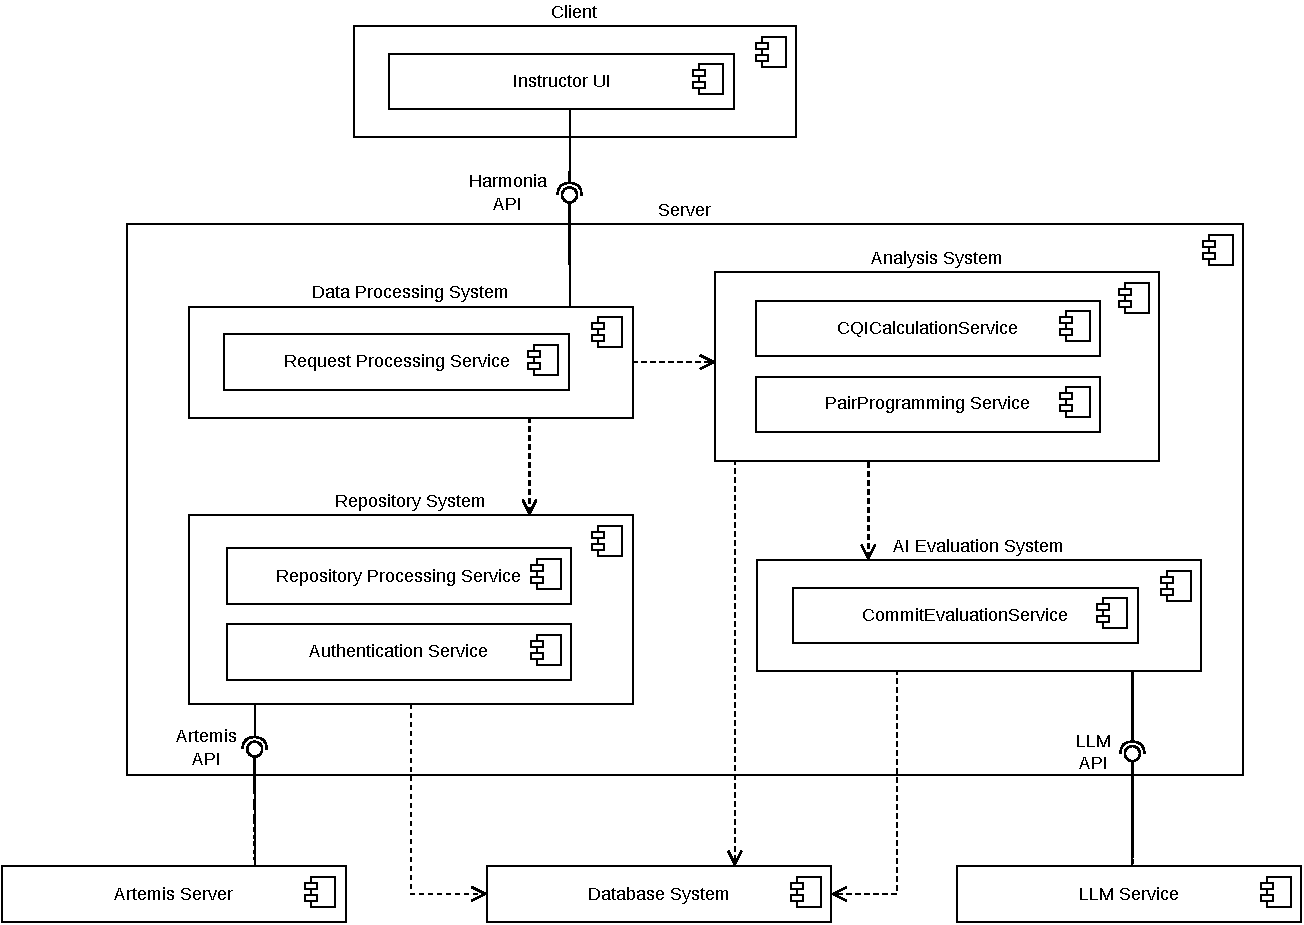
\includegraphics[width=\textwidth]{figures/Subsystem_Decomposition.pdf}
  \caption{Subsystem decomposition of Harmonia.}
  \label{fig:subsystem-decomposition}
\end{figure*}

\subsubsection{Server}

The server organizes its logic into two subsystems. The \textbf{Data Processing System} clones Git repositories from Artemis, extracts commit metadata (author, timestamp, changed files, insertions, deletions) and file ownership via blame analysis, manages authentication, and exposes RESTful endpoints plus a Server-Sent Events (SSE) stream for real-time progress updates. The \textbf{Analysis System} computes the CQI and its sub-components, cross-references pair programming attendance records with commit activity, and communicates with an external LLM to classify commits by type and estimate coding effort. These effort estimates feed back into the CQI computation.

\subsubsection{External Systems}

The \textbf{Artemis Server} provides access to course data, team compositions, Git repositories, and version control access logs through its API, eliminating the need for manual data exports. The \textbf{LLM API} receives commit metadata (message, changed file paths, diff statistics) and returns a classification label, an effort score, and a confidence value for each commit.

\subsubsection{Client}

The client is a single-page web application that serves as the primary interface for instructors and tutors. It communicates with the server exclusively through the REST API and the SSE stream. The interface organizes its functionality around three main views. The \textit{teams overview} provides a course-wide dashboard listing every team with its CQI score, commit count, lines of code, and analysis status; instructors can sort, filter, and compare teams against course-wide averages. The \textit{team detail view} breaks the CQI into its sub-component scores (Effort Balance, LoC Balance, Temporal Spread, Ownership Spread, and Pair Programming) so that instructors can pinpoint which aspects of collaboration are strong or weak. Below the score cards, an \textit{AI analysis feed} lists every commit with its AI-assigned effort rating, category, and lines changed; expanding an entry reveals the full AI reasoning, including complexity, novelty, and confidence, ensuring scoring transparency. During an active analysis, the client updates its state progressively as the SSE stream delivers status changes for each team, allowing instructors to review completed teams without waiting for the full course analysis to finish.

\subsubsection{Database}

Harmonia uses a relational database to persist teams, students, commits, file-level changes, computed scores, and analysis job metadata. Version-controlled migration scripts manage schema evolution. Storing intermediate results allows the client to display partial progress during an ongoing analysis and to retrieve historical results for past exercises.

\subsection{Collaboration Quality Index}
\label{sec:cqi}

The central metric Harmonia produces is the \textbf{Collaboration Quality Index (CQI)}, a composite score between 0 and 100 that quantifies how well a team collaborated during the project by combining multiple dimensions of collaboration.

\subsubsection{Composition}

Harmonia computes the CQI as a weighted sum of four sub-scores, each measuring a different aspect of collaboration:

\begin{equation}
\text{CQI} = w_1 \cdot \text{Effort} + w_2 \cdot \text{LoC} + w_3 \cdot \text{Temporal} + w_4 \cdot \text{Ownership}
\end{equation}

Table~\ref{tab:cqi-components} summarizes the weights $w_1$ through $w_4$ and describes each component. The Effort Balance component carries the largest weight because it accounts for the qualitative importance of contributions. Harmonia uses an AI model to classify each commit and estimate the actual coding effort involved. This mechanism allows the system to distinguish between a commit that introduces a new feature and one that merely reformats existing code.

\subsubsection{Calculation}

The two balance-based components, Effort Balance and LoC Balance, use the \textbf{Gini coefficient} to measure inequality in the distribution of work. A Gini coefficient of zero indicates perfect equality, while a value of one means a single person produced all the work. Harmonia computes the component score as $100 \times (1 - G)$, where $G$ denotes the Gini coefficient, so a perfectly balanced team scores 100 and a team with a single contributor scores 0.

Temporal Spread uses the \textbf{coefficient of variation} (CV), the ratio of standard deviation to mean, over weekly effort totals. A low CV indicates consistent work throughout the project, while a high value signals irregular bursts of activity. Harmonia computes this score as $100 \times (1 - \min(\text{CV} / 5, 1))$. Ownership Spread examines how many distinct authors contributed to each relevant file (files with at least three commits) and computes the average ratio of contributing authors to team size across all such files.

\begin{table}[h]
  \caption{Components of the Collaboration Quality Index.}
  \label{tab:cqi-components}
  \small
  \begin{tabular}{@{}lcl@{}}
    \toprule
    \textbf{Component} & \textbf{Weight} & \textbf{Method} \\
    \midrule
    Effort Balance  & 55\% & Gini over LLM-rated effort \\
    LoC Balance     & 25\% & Gini over lines changed \\
    Temporal Spread &  5\% & CV over weekly effort \\
    Ownership Spread& 15\% & Author/file ratio \\
    \bottomrule
  \end{tabular}
\end{table}

\subsubsection{Edge Cases and Filtering}

Teams with only a single contributor or no productive commits automatically receive a CQI of zero. Before scoring, Harmonia excludes commits that do not represent substantive work: empty commits, merge commits, reverts, rename-only changes, formatting-only edits, mass reformats, changes to generated files, and commits with trivial messages.

\subsubsection{Pair Programming Verification}
\label{sec:pp}

Tutors upload attendance records from mandatory pair programming sessions into Harmonia, which cross-references them with the commit history. For each session, the system checks whether both students made commits on the corresponding day, providing an objective basis for assessing compliance that complements tutor observations.

\subsection{Analysis Pipeline}

The analysis pipeline follows a three-phase architecture that maximizes throughput while providing continuous feedback to the instructor. The first phase, the \textbf{Download Phase}, clones all team repositories in parallel and fetches the corresponding access logs from Artemis. Teams that fail to download receive a failure status without blocking the remaining teams. The second phase, the \textbf{Git Analysis Phase}, processes each downloaded repository in parallel by extracting commit metadata, computing per-author contribution statistics, and determining file ownership. The server persists partial results, including the Git-based sub-scores, and makes them immediately available to the instructor.

The third phase, the \textbf{AI Analysis Phase}, processes each team's commits sequentially through the AI model to classify commit types and estimate effort. The server then computes the final CQI by combining the AI-based scores with the Git-based components from the previous phase. The pipeline handles failures gracefully: if the analysis of an individual team fails at any phase, the server logs the error and continues processing the remaining teams.

\subsection{Implementation Status}

Table~\ref{tab:implementation-status} summarizes the implementation status. The team fulfilled most requirements; the gaps reflect deliberate scope decisions.

\begin{table}[h]
  \caption{Implementation status of Harmonia requirements.}
  \label{tab:implementation-status}
  \begin{tabular}{cll}
    \toprule
    \textbf{ID} & \textbf{Status} & \textbf{Remark} \\
    \midrule
    FR-01 & Fulfilled & \\
    FR-02 & Fulfilled & \\
    FR-03 & Partial & Artemis only \\
    FR-04 & Fulfilled & \\
    FR-05 & Fulfilled & \\
    FR-06 & Fulfilled & \\
    FR-07 & Partial & Manual file upload \\
    FR-08 & Fulfilled & \\
    FR-09 & Fulfilled & \\
    \midrule
    QR-01 & Not fulfilled & 24h vs.\ 15 min target \\
    QR-02 & Fulfilled & \\
    QR-03 & Partial & Not stress-tested \\
    QR-04 & Fulfilled & \\
    QR-05 & Fulfilled & \\
    QR-06 & Not fulfilled & Instructor-only access \\
    \bottomrule
  \end{tabular}
\end{table}

We limited Repository Integration (FR-03) to Artemis because ITP exclusively uses that platform. Pair-Programming Session Logging (FR-07) relies on an externally prepared attendance file rather than in-tool logging. The team descoped Role-Based Access (QR-06) to focus on core analysis capabilities. The largest open gap is Analysis Completion Time (QR-01): sequential AI processing causes the runtime to scale linearly with the number of commits, requiring up to 24 hours for 200 teams. Parallelizing or batching AI requests remains a priority for future optimization.

%% ============================================================
%% SECTION 5: Evaluation of Harmonia
%% ============================================================
\section{Evaluation of Harmonia}

\subsection{Set Up}
We deployed Harmonia with the GPT-5-Mini model and selected five student teams from the ITP winter semester 2025/26 course to compare automated assessments with human judgment. The teams, referred to by pseudonyms, cover a diverse range of outcomes (Table~\ref{tbl:teams}). Team F failed because one member did not meet the minimum commit count; we manually triggered an AI analysis for evaluation purposes.

\begin{table}
  \caption{Overview of the five evaluated teams and their CQI scores.}
  \label{tbl:teams}
  \begin{tabular}{lcl}
    \toprule
    \textbf{Team} & \textbf{CQI Score} & \textbf{Description} \\
    \midrule
    Team H & 98 & Highest score \\
    Team A1 & 92 & Average score \\
    Team A2 & 94 & Average score \\
    Team L & 73 & Lowest passing score \\
    Team F & 92 & Failed (manually analyzed) \\
    \bottomrule
  \end{tabular}
\end{table}

Two independent reviewers manually assessed every Git commit from both team members of each team, classifying each commit into one of four categories: Feature, Bug Fix, Refactor, or Trivial. The reviewers also rated each commit on three dimensions using a scale from 0.0 to 10.0: ``Effort'' captures the amount of meaningful work, ``Complexity'' reflects the technical difficulty of the code changes, and ``Novelty'' measures how much original code the commit introduced rather than boilerplate or duplicated content. Using two independent assessments reduces the risk of individual bias and increases reliability.

\subsection{Results}
We first measured agreement between the two reviewers using the Pearson correlation coefficient (0\%--100\% scale) and computed ``Category'' agreement as the percentage of commits where both reviewers assigned the same category. Figure~\ref{fig:irr} shows the results across all five teams.

\begin{figure*}[h]
  \centering
  
\includegraphics[width=\textwidth]{figures/01_inter_rater_combined.png}
  \caption{Correlation between two manual assessments across all five teams.}
  \label{fig:irr}
\end{figure*}

Most values lie above the 70\% threshold for strong positive correlation. Team A1 shows near-perfect agreement (98\% Effort, 98\% Complexity, 99\% Novelty, 93\% Category), while Team H shows the largest disagreement (average 70\%, Complexity as low as 67\%). The remaining teams show stable agreement above 72\%. These results confirm the manual evaluation is sufficiently consistent to serve as a baseline.

We then compared the average scores assigned by human reviewers with those produced by Harmonia. Figure~\ref{fig:scores} shows the mean ``Effort'', ``Complexity'', and ``Novelty'' scores per team.

\begin{figure*}[h]
  \centering
  
\includegraphics[width=\textwidth]{figures/02_manual_vs_harmonia_scores.png}
  \caption{Average ``Effort'', ``Complexity'', and ``Novelty'' scores per team as assessed by manual reviewers and Harmonia.}
  \label{fig:scores}
\end{figure*}

Harmonia consistently underestimates ``Effort'' relative to human reviewers, with gaps ranging from +0.2 (Team L) to +2.0 (Team A2), suggesting it undervalues meaningful work in higher-quality teams. For ``Complexity'', the pattern reverses: Harmonia rates most teams higher, with the largest gap for Team L (-0.9). ``Novelty'' aligns closely for some teams (Team H: 0.0 difference) but diverges for others (Team A2: +1.5), following a similar pattern as ``Effort''.

Figure~\ref{fig:categories} shows the distribution of commit categories assigned by both the human reviewers and Harmonia.

\begin{figure*}[h]
  \centering
  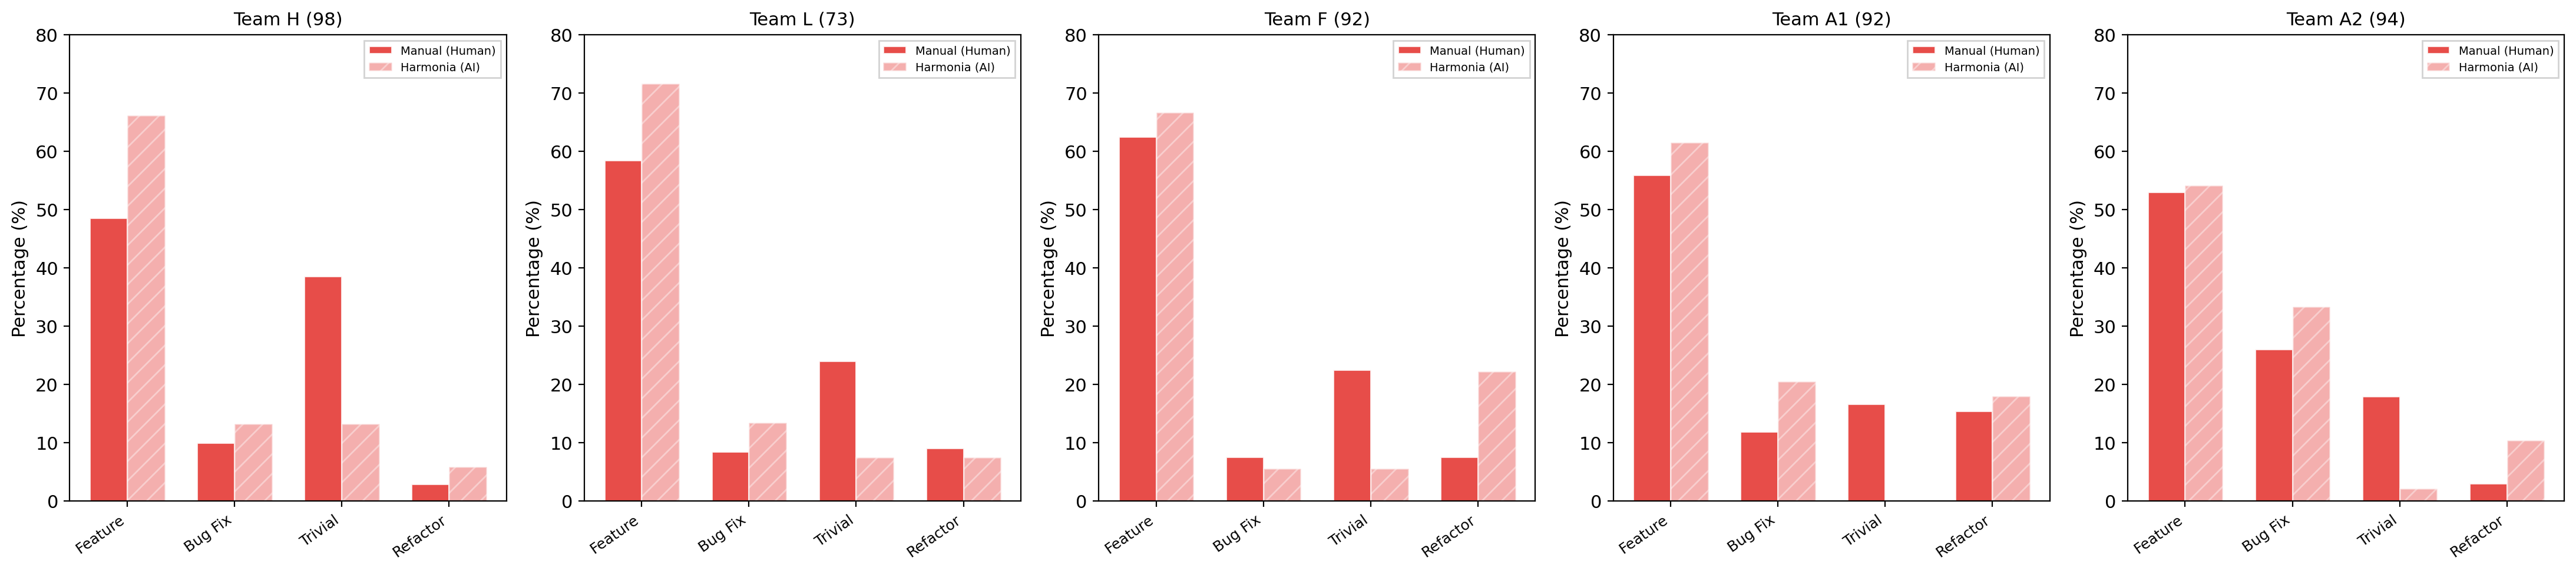
\includegraphics[width=\textwidth]{figures/03_category_distribution.png}
  \caption{Distribution of commit categories as classified by manual assessments and Harmonia.}
  \label{fig:categories}
\end{figure*}

Across all teams, Harmonia overclassifies commits as ``Feature'' (e.g., 66\% vs.\ 48\% human for Team H) and ``Bug Fix'' while systematically underclassifying ``Trivial'' commits (e.g., 13\% vs.\ 39\% human for Team H; 0\% vs.\ 18\% for Team A1). This shift from ``Trivial'' into ``Feature'' and ``Bug Fix'' is consistent across all analyzed teams.

At the individual commit level, manual scores fluctuate sharply from commit to commit across all teams, with the three dimensions remaining closely aligned (average absolute difference of 0.5--0.6 points). A per-commit comparison of Team H (lowest inter-rater agreement) and Team A1 (highest agreement) with Harmonia reveals that Harmonia operates within a compressed scoring range of roughly 0.5 to 5.0, while human reviewers use the full 0.0--10.0 scale. Despite this compression, Harmonia's relative patterns track the human assessments: commits rated high by both reviewers also receive higher scores from Harmonia, though the absolute values remain much lower. The gap between human and AI scores is more pronounced for Team A1, consistent with its higher manual averages.

\subsection{Limitations}
The evaluation carries several limitations. The sample of five teams restricts generalizability; a larger study would strengthen the conclusions. The manual assessment introduces subjectivity: reviewers may favor commits with longer messages, classify commits based on explicit category mentions rather than inspecting code, or penalize suspected AI-generated code. Inter-rater reliability ranges from 68\% to 99\% depending on team and dimension. Multi-purpose commits that combine, for example, refactoring with a new feature make single-category assignment inherently ambiguous. More broadly, no objectively correct score exists for any commit. Both human and AI classifications represent interpretations, and disagreement does not necessarily indicate error on either side.

On the AI side, Harmonia's compressed scoring range (0.5--5.0 vs.\ the human 0.0--10.0 scale) makes absolute comparison difficult even when relative patterns align. Harmonia also systematically underclassifies ``Trivial'' commits. The results depend on the specific model (GPT-5-Mini); a different model could produce different scores and classifications.

%% ============================================================
%% SECTION 6: Student View
%% ============================================================
\section{Student View}
\label{sec:student_view}

Harmonia addresses the instructor's assessment and transparency challenge, but students themselves also benefit from support during development. Delivering discrete, summative feedback only at project submission offers limited opportunity for learning and improvement. This section presents a complementary system that delivers formative feedback to students in real time through large language models, enabling continuous code quality assessment and iteration.

The student feedback system provides low-friction access to code quality critique throughout the project lifecycle. By integrating with the course's online development environment ``Artemis'', it removes barriers to feedback requests and presents guidance at the moment of need. The system frames all feedback as non-graded, constructive guidance, encouraging students to seek critique without apprehension and to engage more deeply with code quality principles.

\subsection{Requirements Analysis}

The student feedback system operates under different design principles than Harmonia. While Harmonia produces grading-oriented metrics, the feedback system prioritizes learning support through actionable, balanced critique delivered in real time. Table~\ref{tab:student-functional-requirements} and Table~\ref{tab:student-quality-requirements} list the functional and quality requirements.

\begin{table}[h]
  \caption{Functional requirements for the student feedback system.}
  \label{tab:student-functional-requirements}
  \begin{tabular}{cl}
    \toprule
    \textbf{ID} & \textbf{Requirement} \\
    \midrule
    FR-01 & Request Feedback Button \\
    FR-02 & Repository Retrieval \\
    FR-03 & Analysis Execution \\
    FR-04 & Feedback Generation \\
    FR-05 & Feedback Display \\
    FR-06 & Unscored Assessment \\
    \bottomrule
  \end{tabular}
\end{table}

Students initiate code quality assessment on demand via a button in Artemis (FR-01); the system automatically fetches the current repository state (FR-02) and processes it through an LLM that evaluates code quality, design patterns, and adherence to learning objectives (FR-03). The system categorizes feedback into four priority tiers, namely critical, major, minor, and nice to have (FR-04), and presents it both as a color-coded aggregated list and as interactive inline annotations at the exact lines of code within Artemis' online IDE (FR-05). All feedback carries an explicit non-graded educational guidance designation (FR-06).

\begin{table}[h]
  \caption{Quality requirements for the student feedback system.}
  \label{tab:student-quality-requirements}
  \begin{tabular}{cl}
    \toprule
    \textbf{ID} & \textbf{Requirement} \\
    \midrule
    QR-01 & Performance ($<$5 min) \\
    QR-02 & Scalability \\
    QR-03 & Reliability \\
    QR-04 & Usability \\
    QR-05 & Maintainability \\
    QR-06 & Understandability \\
    \bottomrule
  \end{tabular}
\end{table}

\subsection{System Design}

The student feedback system introduces a specialized assessment module within Athena, the AI-based assessment platform already integrated with the learning management system~\cite{soelch2026scaling}, reusing established deployment patterns while adding code quality evaluation capabilities. The system comprises three core functional units (Figure~\ref{fig:student-view-architecture}).

The \textbf{Request Interface} takes the form of a button within the exercise details view of Artemis. When a student clicks it, the system captures the repository state, specifically the diff between the student's implementation and the problem template, and routes it to the analysis pipeline.

The \textbf{Analysis Engine} runs as a containerized Athena module written in Python and executed in Docker. The module constructs a unified diff against the reference template, then assembles a prompt containing the problem statement, coding standards, and the diff. The prompt instructs the LLM to adopt the perspective of a human tutor unfamiliar with official solutions and to balance feedback. The LLM returns structured feedback that the module parses and organizes into priority categories.

The system grounds all feedback in specific code locations and diffs, tying suggestions directly to the student's work. Suggestions target principles, code organization, and design patterns rather than prescribing specific implementations, reinforcing the goal that students develop independent problem-solving skills.

\begin{figure*}[h]
  \centering
  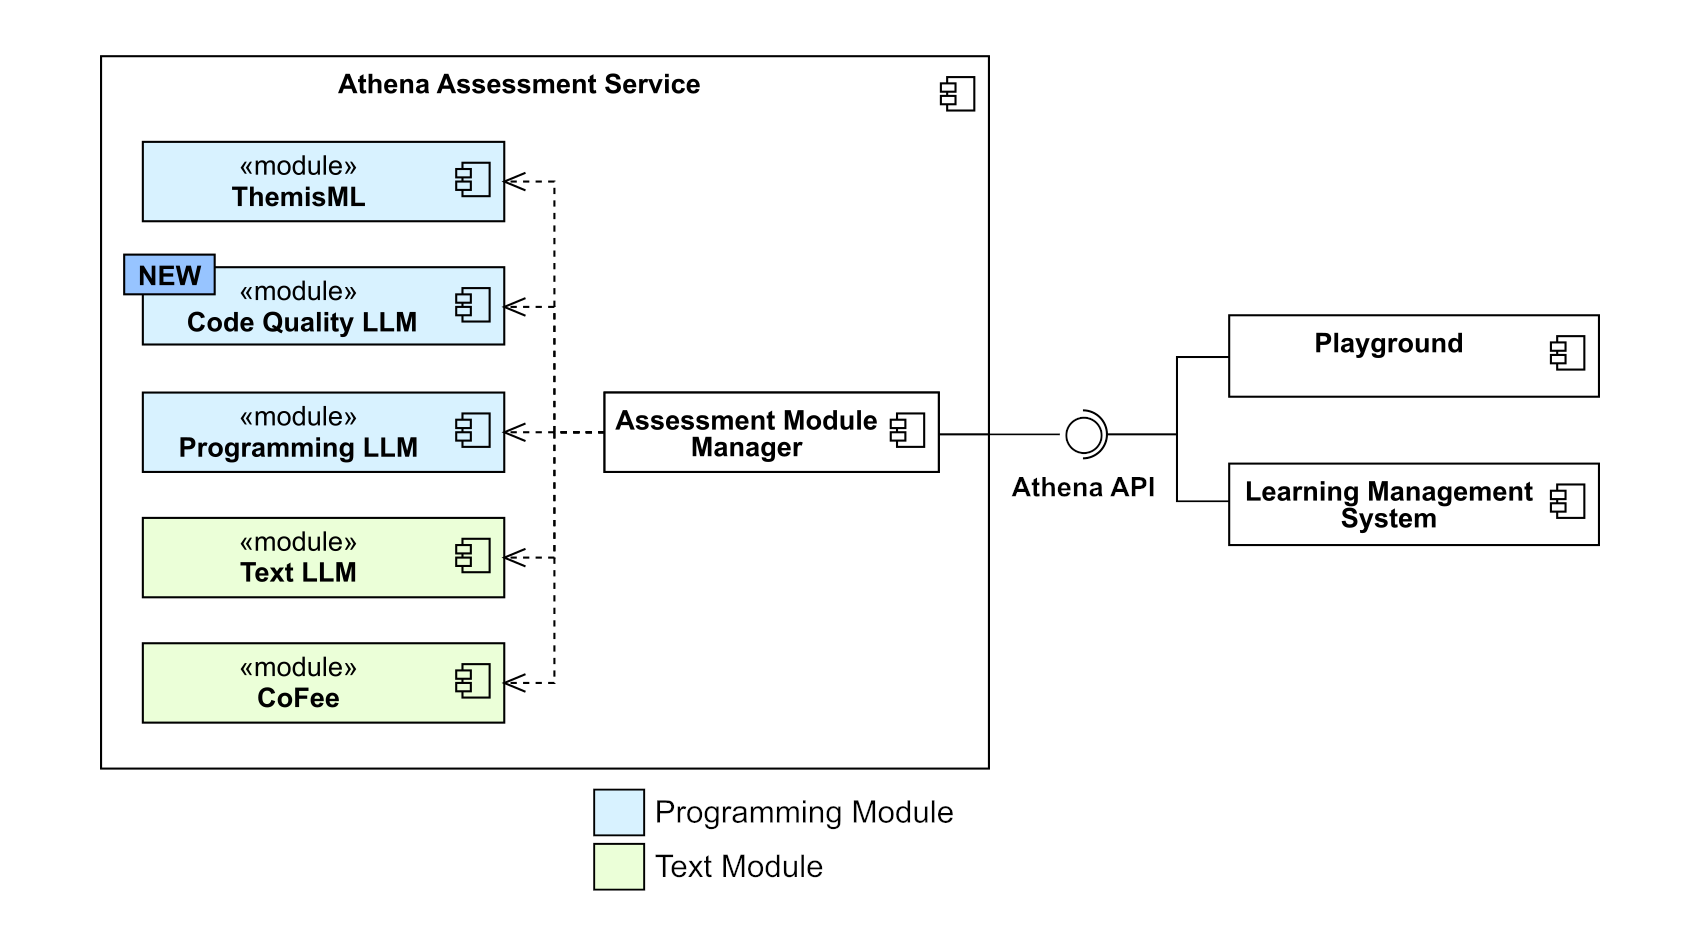
\includegraphics[width=\textwidth]{figures/student_view_architecture.png}
  \caption{Athena Assessment Service architecture showing the Code Quality LLM module alongside other assessment modules, managed by the Assessment Module Manager and accessed via the Athena API.}
  \label{fig:student-view-architecture}
\end{figure*}

\subsection{Feedback Taxonomy}

The system classifies all feedback into one of four priority categories. A \textbf{Critical Issue} denotes defects that compromise correctness or safety, such as security vulnerabilities, runtime crashes, data loss, or incorrect output, and students must resolve these before submission. A \textbf{Major Issue} covers substantial code quality degradations, performance bottlenecks, or deviations from coding standards. A \textbf{Minor Issue} refers to code smells, non-critical style violations, or readability enhancements worth considering as time allows. A \textbf{Nice to Have} marks stylistic refinements or optional improvements that do not affect functionality. Each feedback item carries its priority as a prefix, enabling students to focus first on the most impactful improvements.

\subsection{Implementation Status}

Table~\ref{tab:student-implementation-status} summarizes the implementation status. We have implemented and technically integrated the system, but it has not yet run in a live course; we have prepared it for deployment in future iterations.

\begin{table}[h]
  \caption{Implementation status of student feedback system.}
  \label{tab:student-implementation-status}
  \begin{tabular}{cll}
    \toprule
    \textbf{ID} & \textbf{Status} & \textbf{Remark} \\
    \midrule
    FR-01--06 & Fulfilled & \\
    QR-01--05 & Fulfilled & \\
    QR-06 & Not Fulfilled & Needs simpler language \\
    \bottomrule
  \end{tabular}
\end{table}

The system supports student learning during development through timely, non-graded feedback and a clear priority taxonomy for issue triage. We will evaluate its effectiveness in future course iterations once students use it in practice. Beyond the current course context, the architecture and module design also enable transfer to other courses with similar programming assessment needs.

%% ============================================================
%% SECTION 7: Conclusion
%% ============================================================
\section{Conclusion}

This paper presented Harmonia, a system for automated assessment of student collaboration in team software projects. The Collaboration Quality Index (CQI) combines LLM-rated effort (55\%), lines of code balance (25\%), temporal spread (5\%), and file ownership (15\%) into a composite metric that moves beyond commit counts to assess the semantic quality of contributions. We deployed Harmonia in ITP for winter semester 2025/26 and validated it through manual evaluation of five teams, which showed inter-rater reliability above 70\% on effort, complexity, and novelty dimensions, indicating that human and LLM assessments operate within a comparable range of variability.

The system also exposes limitations. The CQI can obscure qualitative differences, as a high-scoring team might have divided responsibilities despite balanced effort. The sequential AI analysis scales linearly with commits, requiring 24 hours for 200 teams, which far exceeds the 15-minute target. Git history captures authorship and timestamps but not actual time invested, meaning that commits pushed by one student may represent joint collaboration. The student feedback system complements instructor assessment by delivering non-graded, priority-categorized feedback in real time, removing grading anxiety and supporting learning throughout development.

The two-sided approach, summative assessment for instructors and formative guidance for students, demonstrates how LLM-driven tools can support different stakeholders in team-based courses. Whether effort estimation generalizes to other LLM providers, and how to detect intentional gaming of the metric, remain open questions.

%% ============================================================
%% SECTION 8: Future Work
%% ============================================================
\section{Future Work}
This section outlines directions for extending Harmonia and the student feedback system beyond their current capabilities.

\subsection{Tutor View}

Harmonia currently requires instructors to upload pair programming attendance records as external files, which tutors must prepare manually outside the system. A dedicated tutor view would allow tutors to log pair programming sessions directly within Harmonia, selecting the date, duration, and attendees for each session. The system would then associate commits within the logged time window automatically, replacing the manual file-based workflow. The tutor view would also provide each tutor with a dashboard displaying only their assigned teams with metrics such as CQI scores, commit counts, and collaboration status, giving tutors direct visibility into their teams' progress. A role-based login would restrict each tutor's view to their own teams, addressing the currently unfulfilled Role-Based Access requirement (QR-06).

\subsection{Code Quality Score}

The student feedback system currently presents all feedback as ungraded guidance. A future extension could introduce a Code Quality Score that aggregates the priority-categorized feedback items into a single numeric value. Unlike the CQI, which measures collaboration and targets instructors, the Code Quality Score would target students and reflect code-level concerns such as correctness, style, and design. Offering a score creates a middle ground between completely ungraded feedback and formal assessment, motivating students to iterate on their code while preserving the non-punitive character of the feedback system.

\subsection{Performance and Analysis Time}

The sequential AI analysis phase forms the primary bottleneck, with full course analysis requiring up to 24 hours for 200 teams. Batching commit requests to the LLM API in parallel rather than processing them sequentially could reduce this overhead. A hybrid approach that applies fast heuristics for obvious cases such as formatting-only changes and merge commits, and routes only ambiguous commits to the LLM, could further accelerate processing while maintaining assessment quality.

\subsection{Platform Integration and Portability}

Harmonia currently integrates exclusively with Artemis due to ITP's platform choice. Implementing GitLab and GitHub support would enable adoption in institutions using those platforms. Defining a standardized export format for CQI scores and collaboration evidence would also facilitate integration with other grading systems and research tools, reducing dependence on platform-specific implementations.

%% ============================================================
%% Transparency: AI Tools
%% ============================================================
\section*{Transparency: Use of AI Tools}
In preparing this paper, we used Grammarly for grammar and style corrections across all sections to ensure clarity and coherence. We employed DeepL to improve language quality and to translate parts of the Literature Review. We used AI assistants such as ChatGPT and Claude to help generate initial drafts, refine ideas, and provide suggestions across all sections of the paper. Furthermore, we used AI-based coding tools such as GitHub Copilot to assist with code generation for both Harmonia and the student feedback system. We thoroughly reviewed and verified all content produced with the aid of these tools for correctness and coherence.

\bibliographystyle{ACM-Reference-Format}
\bibliography{references}

\end{document}
